\section{表面あらさ計測(大野・奥山)}
\label{chap:surfaceroughness}

\subsection{計測の目的}

第\ref{chap:shapemeasurement}章で述べたように,衛星のレールはICDにより表面粗さをRa1.6 $\mu$m以下とするように規定されている.しかし,本衛星の側面パネルを発注した際に,誤って図面での表面粗さ指定をRa6.3 $\mu$mとしてしまった.そのため,要求を満たしているか確認するために表面粗さ計測試験を行った.

\subsection{計測機器}

表面粗さ計測には以下の図\ref{fig:surfaceroughness}のような東工大工場にある表面粗さ計測機を用いた.

\begin{figure}[h]
	\begin{center}
		
		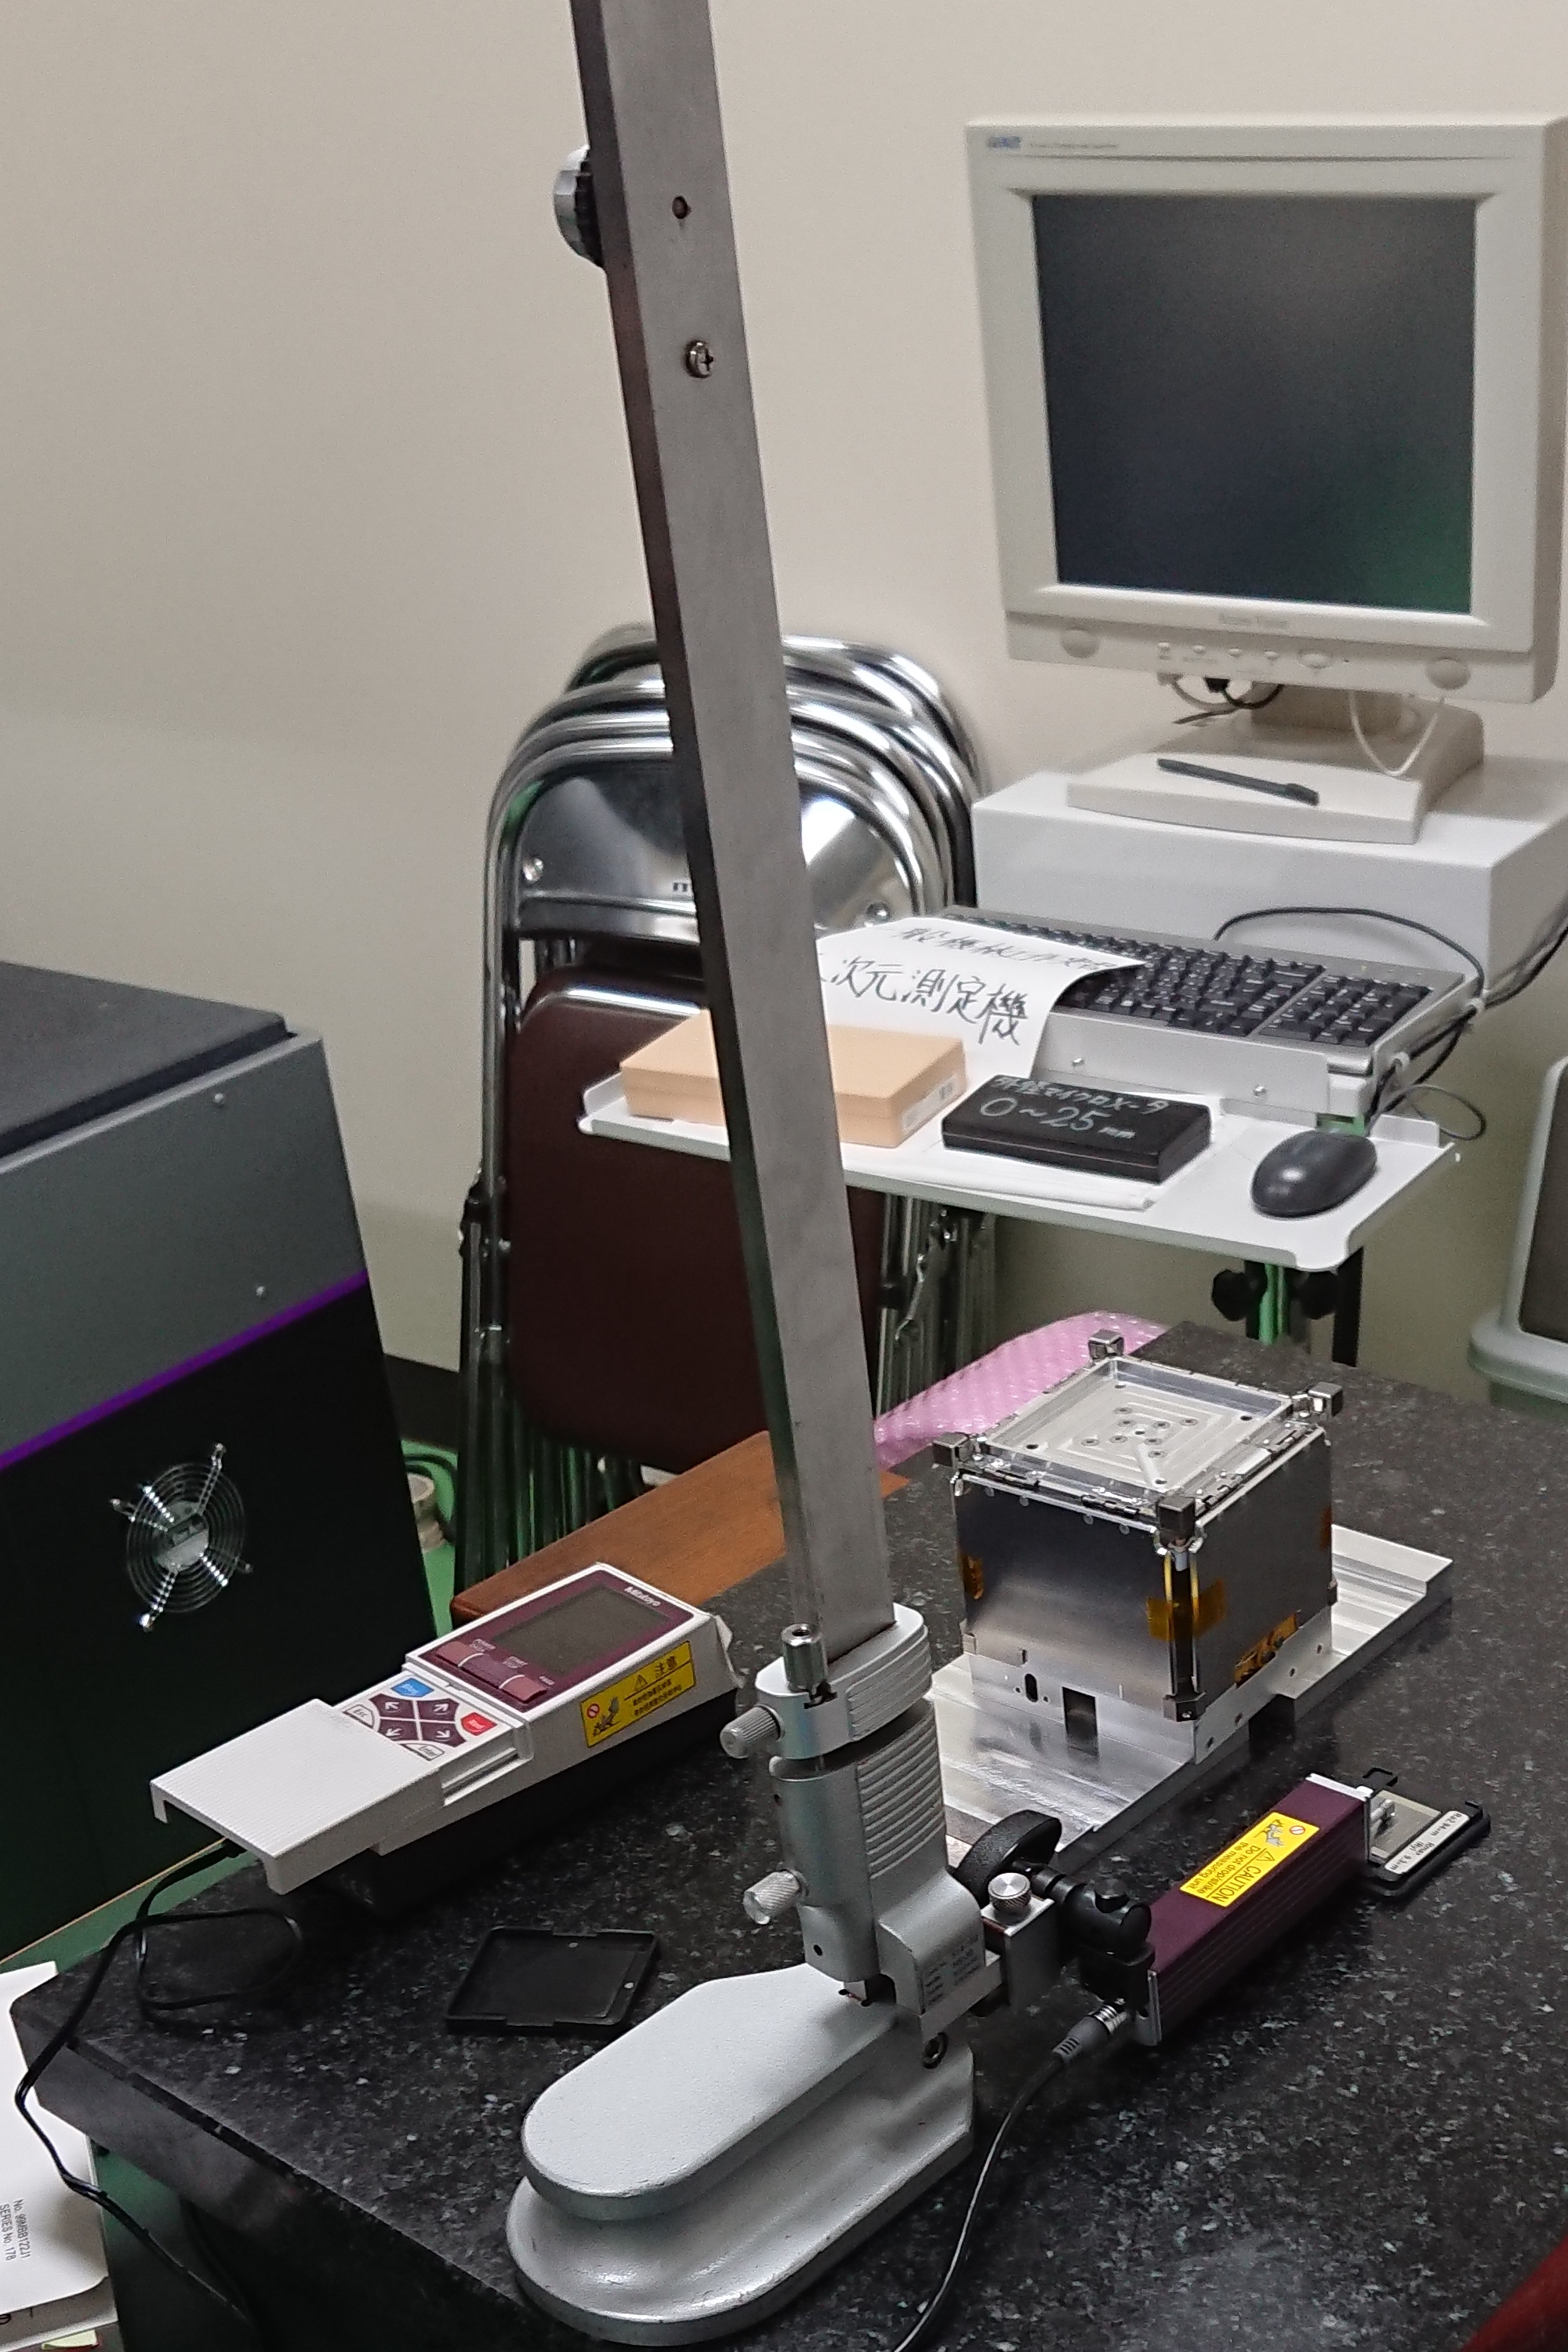
\includegraphics[width=0.3\linewidth]{04/fig/surfaceroughness.jpg}
		\caption{表面粗さ計測機}
		\label{fig:surfaceroughness}
		
	\end{center}
\end{figure}

表面粗さ計測機も第\ref{chap:shapemeasurement}章で述べた三次元測定機と同様に,工場特殊セルフ利用に該当するため,講習を受けたのちに教員の立会いのもと用いることができる.

\subsection{1回目の計測}

図面では誤った表面粗さ指定をしてしまっていたが,実際の数値を確かめるためにレール各部の表面粗さ計測を行った.膜展開部については各面1点ずつ,側面パネルについては各面5点ずつ,底面パネルについては各面2点ずつ行った.その結果,図面での指定を間違えていたものの多くの点で要求を満たしていた.しかし,以下の図\ref{fig:scratch1}に示すように膜展開部,側面パネルのレールの一部に傷がついており,傷の部分で要求を満たしていなかった.詳しい試験結果は「表面粗さ測定結果」を参照のこと.

\begin{figure}[h]
	\begin{center}
		
		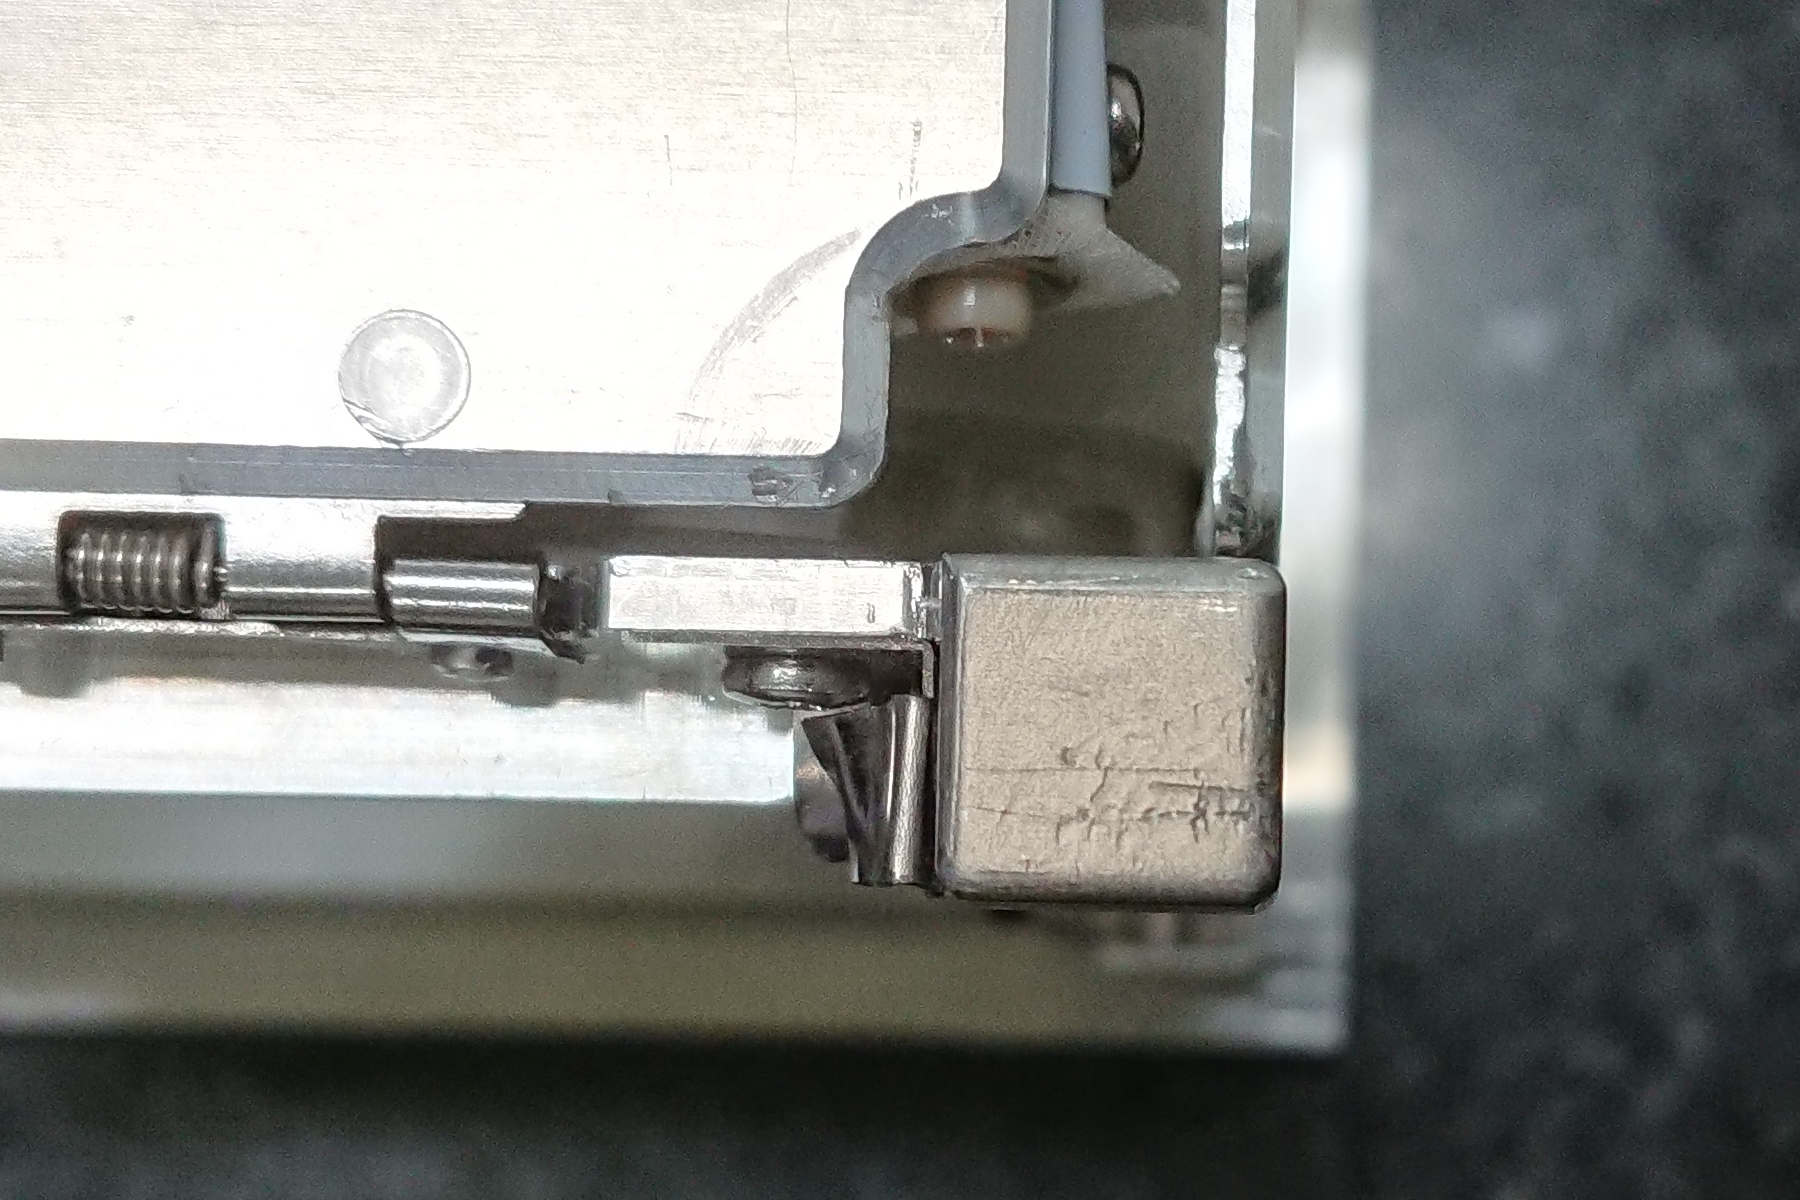
\includegraphics[width=0.6\linewidth]{04/fig/scratch1.jpg}
		\caption{幕展開部レールの傷}
		\label{fig:scratch1}
		
	\end{center}
\end{figure}

\begin{figure}[h]
	\begin{center}
		
		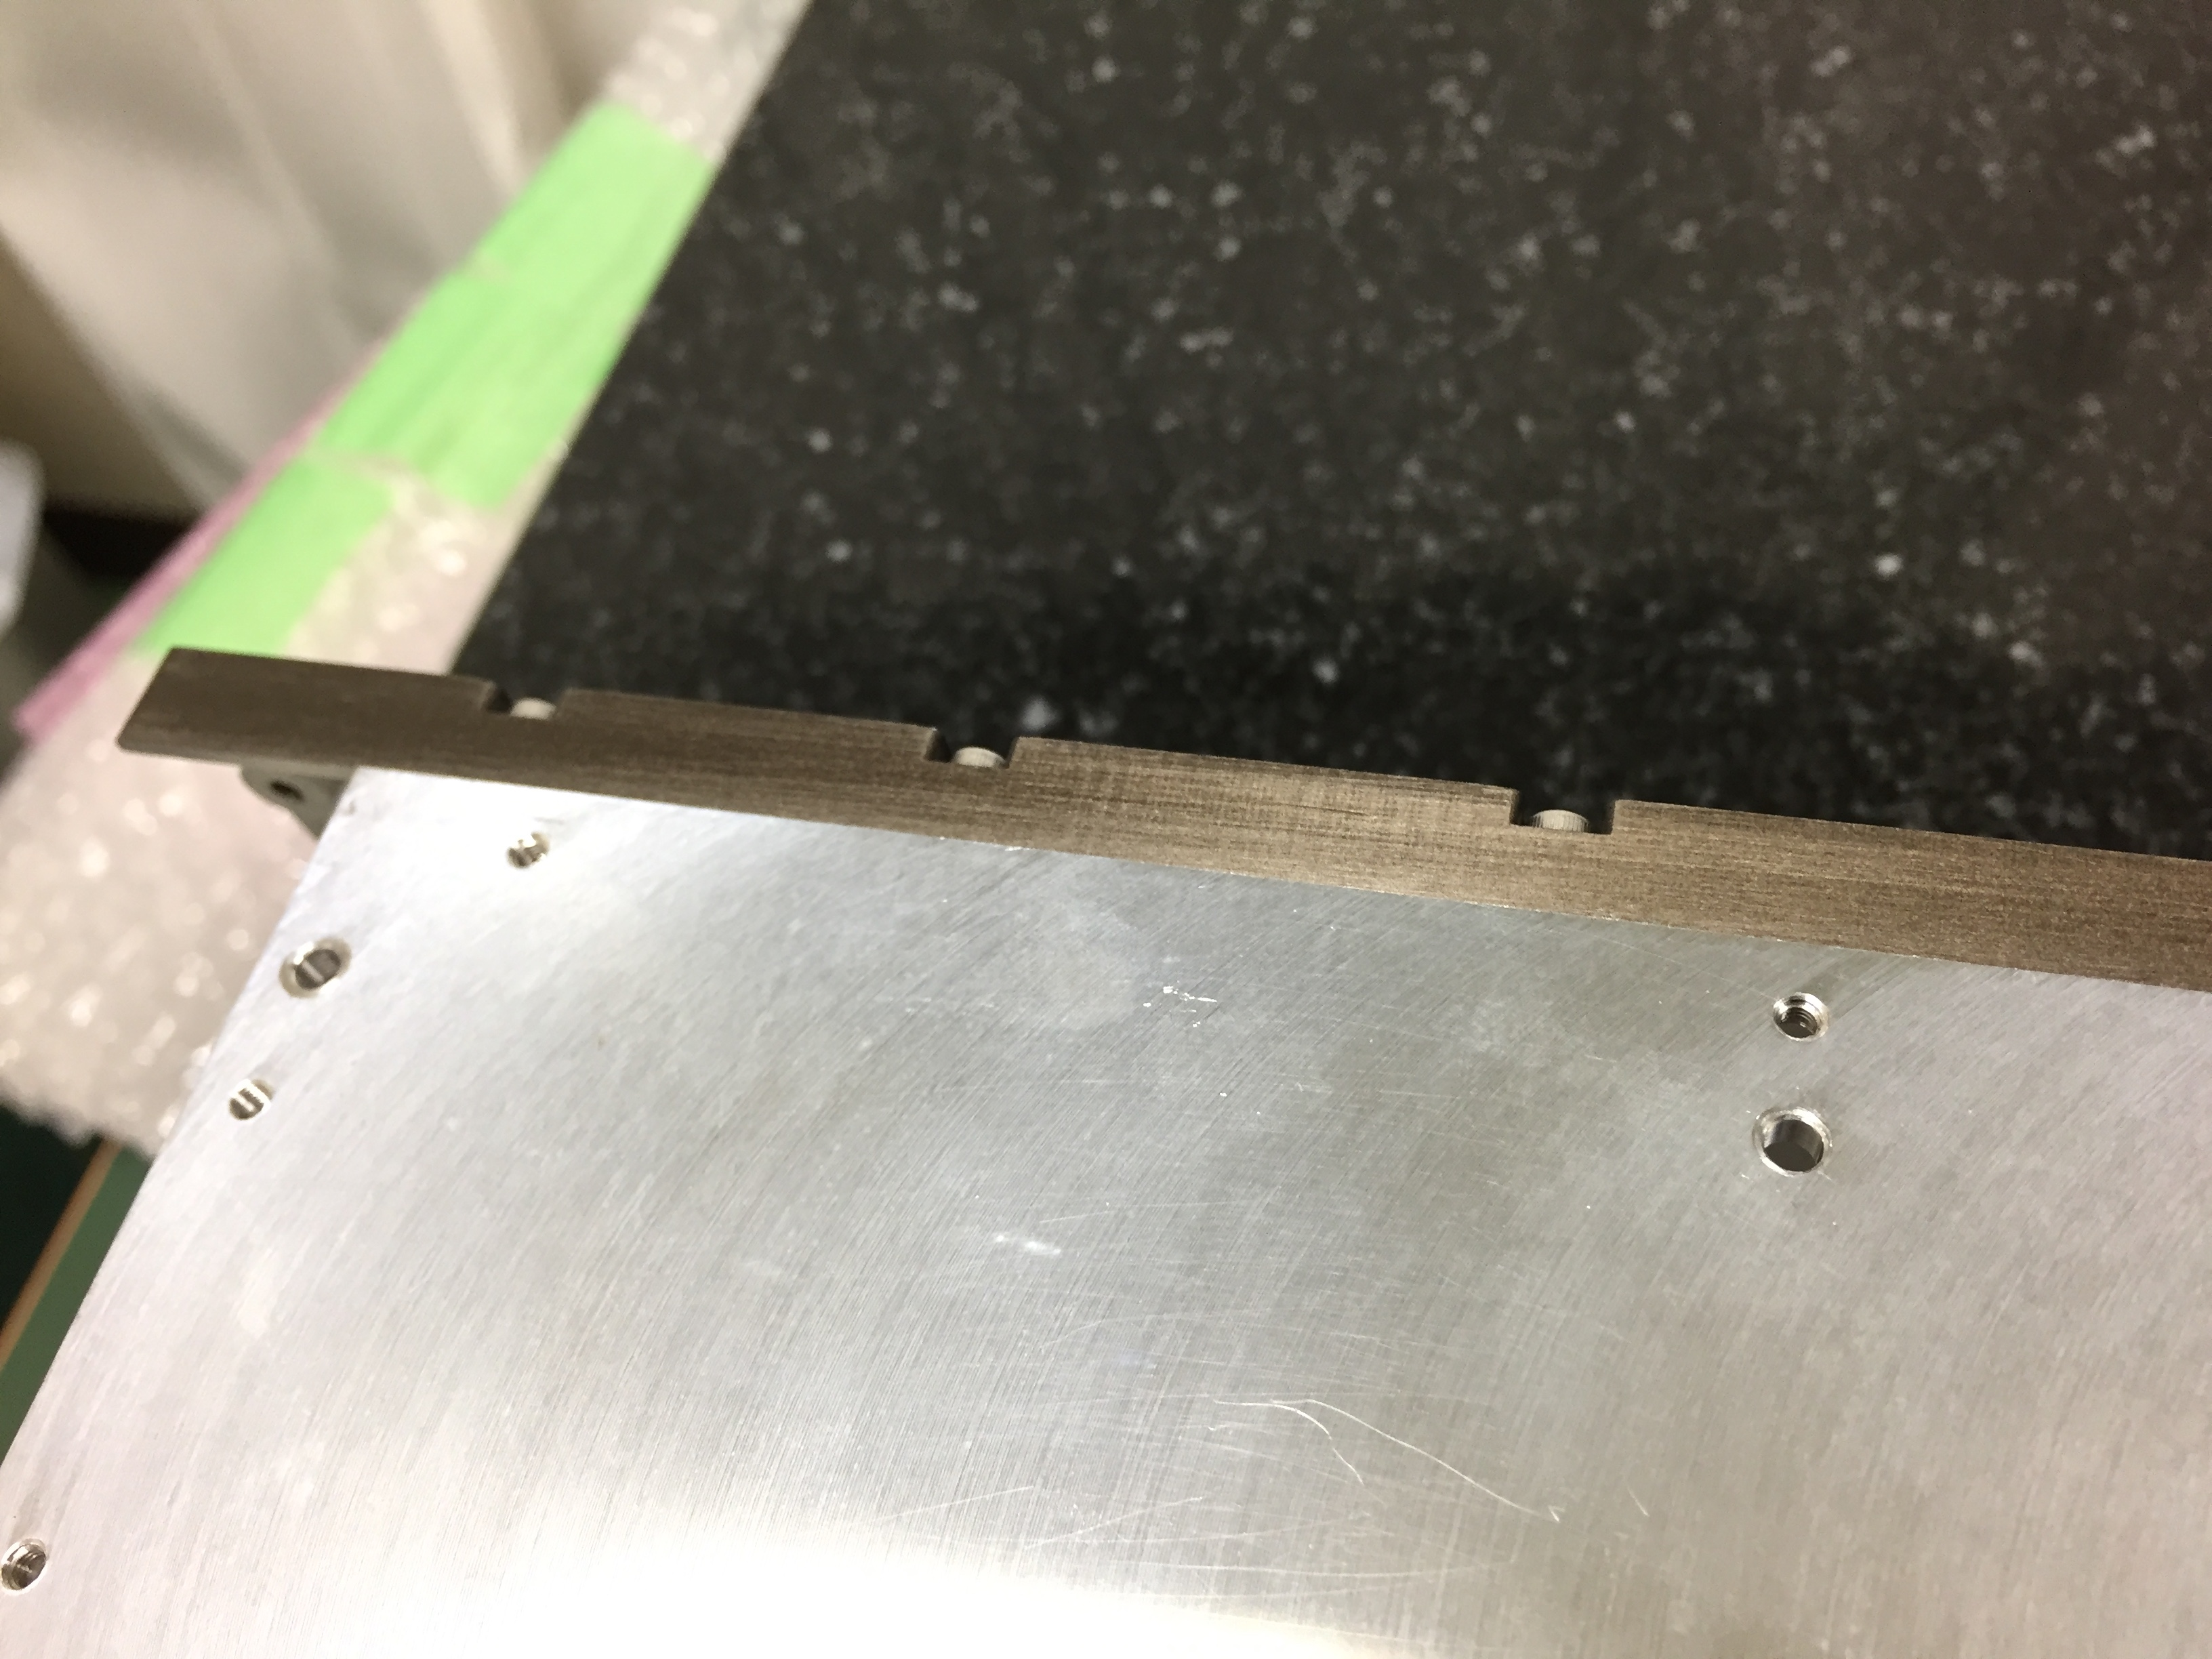
\includegraphics[width=0.6\linewidth]{04/fig/scratch2.jpg}
		\caption{側面パネルレールの傷}
		\label{fig:scratch2}
		
	\end{center}
\end{figure}

\subsection{レール傷の処理}

レールに傷がつくと表面粗さに影響するため,組み立て時に傷がつくことを防ぐ必要がある.そのため,組み立て時に用いた治具のレール部に精度出しを行う時以外にはカプトンテープを貼って保護する,膜展開部のレールは,精度出し以外の時にカプトンテープを貼って保護するという対策を行った.側面パネルX-については,表面粗さが規定を超えていた部分を削り表面を滑らかにした.しかし,以下の図\ref{fig:scrape}のようにハードアノダイズド処理された部分まで削ってしまった.そのため,再度ハードアノダイズド処理を行った.

\begin{figure}[h]
	\begin{center}
		
		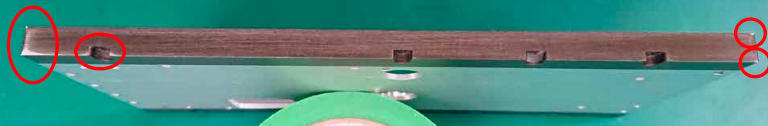
\includegraphics[width=0.8\linewidth]{04/fig/scrape.png}
		\caption{側面パネルレールのハードアノダイズド処理の欠損}
		\label{fig:scrape}
		
	\end{center}
\end{figure}

\subsection{2回目の計測}

再ハードアノダイズド処理を施したX-側面パネルレールの表面粗さを計測すると,要求を満たしていた.詳しい試験結果は「表面粗さ測定結果(再ハードアノダイズド処理後)」を参照のこと.